\documentclass[12pt]{article}
\usepackage{epsfig}
\usepackage{amsmath}
\usepackage{amssymb}
\usepackage{amsfonts}
\usepackage{multirow}
\usepackage{graphicx}
\parindent 30pt\textheight 22cm\topmargin 0in\textwidth 16cm
\oddsidemargin .25in\evensidemargin 0in
\baselineskip=16pt
\def\be{\begin{eqnarray}}\def\ba{\begin{eqnarray}}
\def\ee{\end{eqnarray}}\def\ea{\end{eqnarray}}
\def\ben{\begin{enumerate}}\def\bitem{\begin{itemize}}
\def\een{\end{enumerate}}\def\eitem{\end{itemize}}
\def\no{\nonumber\\}
\def\ie{{\it i.e}}\def\bi{\bibitem}
\def\etal{{\it et. al.}}
%\def\Kp{$K^+$}\def\Km{$K^-$}
\def\Kp{K^+}\def\Km{K^-}
\def\calL{{\cal L}}\def\calF{{\cal F}}
\def\calO{{\cal O}}\def\calR{{\cal R}}
\def\calM{{\cal M}}\def\Gnot{$G_0^\prime$}\def\gnot{$g_0^\prime$}
\def\prl{Phys. Rev. Lett.}\def\pr{Phys. Rev.}\def\np{Nucl. Phys.}
\def\pl{Phys. Lett.}
\def\J#1#2#3#4{ {#1} {\bf #2} {#3} {(#4)} }
\def\PRL{Phys. Rev. Lett.}\def\PL{Phys. Lett.}
\def\PLB{Phys. Lett. B}\def\NP{Nucl. Phys.}
\def\NPA{Nucl. Phys. A}\def\NPB{Nucl. Phys. B}
\def\PR{Phys. Rev.}\def\PRC{Phys. Rev. C}
\def\chibar{{\bar {\chi}}}\def\bfpbar{{\bar {\bf p}}}
\def\na{{\stackrel{\rightarrow}\nabla}}
\def\bfA{{\bf A}}\def\bfJ{{\bf J}}
\def\bfsigma{{\bf \sigma}}
\def\bfk{{\bf k}}\def\bfp{{\bf p}}\def\bfP{{\bf P}}
\def\bfq{{\bf q}}\def\bfx{{\bf x}}\def\bfr{{\bf r}}
\def\bfR{{\bf R}}\def\bfs{{\bf s}}\def\Tr{{\mbox{Tr}}}
\newcommand{\e}{{\mbox{e}}}\def\mN{m_N}\def\del{\partial}
\def\vr{{\vec r}}\def\vk{{\vec k}}\def\vq{{\vec q}}
\def\vp{{\vec p}}\def\vP{{\vec P}}\def\vbp{{\vec {\bar p}}}
\def\vt{{\vec \tau}}\def\vs{{\vec \sigma}}\def\vJ{{\vec J}}
\def\hatc{{\hat c}}\def\hatr{{\hat r}}\def\hatz{{\hat z}}
\def\roughly#1{\mathrel{\raise.3ex\hbox{$#1$\kern-.75em%
\lower1ex\hbox{$\sim$}}}}\def\lsim{\roughly<}
\def\gsim{\roughly>}\def\fm{{\mbox{fm}}}
\def\MeV{{\mbox{MeV}}}\def\erf{{\mbox{erf}}}
\def\erfc{{\mbox{erfc}}}\def\ve{\varepsilon}
\def\calV{{\cal V}}\def\H#1{{}^{#1}\mbox{H}}
\def\He#1{{}^{#1}\mbox{He}}\def\B#1{{}^{#1}\mbox{B}}
\def\ssij{\sigma_i\cdot\sigma_j}
\def\ttij{\tau_i\cdot\tau_j}\def\LS{{\bf L}\cdot{\bf S}}
\def\const{\mbox{const.}}\def\up{\uparrow}
\def\down{\downarrow}\def\nlo#1{\mbox{N$^{#1}$LO}}
\def\vA{{\vec A}}\def\vtau{{\vec \tau}}
\def\zint{{\int_0^1\!dz\,}}\def\zz{{z {\bar z}}}
\def\calR{{\cal R}}\def\caL{{\cal L}}
\def\calN{{\cal N}}
\def\Sunit{10^{-20}\ \mbox{KeV-b}}
\def\tv{{\tilde v}}\def\vx{{\vec x}}\def\vy{{\vec y}}
\def\oO{{\cal O}}\def\oT{{\cal T}}\def\okin{\oO_{{\cal P}}}
\def\FT#1{\left[#1\right]_{\rm FT}}
\def\FTT#1{\left[#1\right]_{\rm FT}^T}
\def\itt{\indent\indent}
\def\E{{\cal E}}
\def\Jb{\mbox{\boldmath$ J$}}\def\Kb{\mbox{\boldmath$ K$}}
\def\Pb{\mbox{\boldmath$ P$}}
\def\Vb{\mbox{\boldmath$ V$}}
\def\Ab{\mbox{\boldmath$ A$}}
\def\jb{\mbox{\boldmath$ j$}}
\def\pb{\mbox{\boldmath$ p$}}\def\qb{\mbox{\boldmath $q$}}
\def\tb{\mbox{\boldmath$ t$}}
\def\ub{\mbox{\boldmath$ u$}} \def\vb{\mbox{\boldmath$ v$}}
\def\xb{\mbox{\boldmath$ x$}}
\def\Bp{\mbox{\boldmath$ p$}}\def\Bq{\mbox{\boldmath $q$}}
\def\Bk{\mbox{\boldmath$ k$}}\def\Br{\mbox{\boldmath $r$}}
\def\Bs{\mbox{\boldmath $s$}}
\def\qbhat{\mbox{\boldmath $\hat{q}$}}\def\taub{\mbox{\boldmath $\tau$}}
\def\pbhat{\mbox{\boldmath $\hat{p}$}}
\def\pbbhat{\mbox{\boldmath $\hat{\bar{p}}$}}
\def\pib{\mbox{\boldmath $\pi$}}
\def\kbhat{\mbox{\boldmath $\hat{k}$}}
\def\nubhat{\mbox{\boldmath $\hat{\nu}$}}
\def\ubhat{\mbox{\boldmath $\hat{u}$}}
\def\gammab{\mbox{\boldmath $\gamma$}}
\def\kappab{\mbox{\boldmath $\kappa$}}
\def\sigmab{\mbox{\boldmath $\sigma$}}
\def\thetab{\mbox{\boldmath $\theta$}}
\def\Tr{{\mathrm Tr}}
\def\Bnabla{\mbox{\boldmath $\nabla$}}
\def\Bsigma{\mbox{\boldmath $\sigma$}}
\def\BSigma{\mbox{\boldmath $\Sigma$}}
\def\Beta{\mbox{\boldmath $\eta$}}
\def\A0{A_0}
\def\bq{\begin{equation}}
\def\eq{\end{equation}}
\def\la{\langle}\def\ra{\rangle}
\def\Km{K^-}\def\Kp{K^+}\def\K0{K^0}
\def\lrarrow {\stackrel{\leftrightarrow}{{\partial}}_\mu}
\def\lrarrowu{\stackrel{\leftrightarrow}{{\partial^\mu}}}

\input{latexdefs.tex}

%\renewcommand{\thefootnote}{\fnsymbol{footnote}}
\renewcommand{\thefootnote}{\arabic{footnote}}
\setcounter{footnote}{0}

\begin{document}
\begin{titlepage}
\begin{center}

 \vskip 1.5cm

{\Large \bf M2-brane, Chern-Simons Theory and Three-Algebras }
\vskip 1. cm
  { Mark van Raamsdonk}

\vskip 0.5cm

{\it Department of Physics \& Astronomy, University of British Columbia\\
6224 Agricultural Road, Vancouver, B.C. V6T 1Z1, Canada }
%{\it UBC}

\end{center}

\centerline{(\today) }
\vskip 1cm
\vspace{1.0cm plus 0.5cm minus 0.5cm}

\begin{abstract}
This paper is a series of lectures given at the 2008 Particles, Fields, $\&$ Strings Summer School at the University of British Columbia.
The lectures aimed to present an introduction to M-theory with a focus mainly on the M2-branes, 
an overview of 2+1 Chern-Simons theory as a candidate for a field theory living on the M2-branes whose proposed gravitational dual would be M-theory on $AdS_4 \times S^7$, 
and to provide a brief review of recent use of Three-Algebras in building a possible Lagrangian satisfying the stringent 
requirements which a field theory on the M2-branes must obey.
\end{abstract}

\end{titlepage}

\newpage


\section{Introduction}

$\qquad \,\,\,$ There has been in the recent months a vast concerted effort, paid off with further progress, in finding an explicit description of low energy world volume physics of multiple coincident M2 branes in M-theory. More familiar for our future considerations would be a stack of N-coincident D branes, extended objects in string theory, whose fluctuations in the large N limit are described by gauge fields, scalars and fermions seen as living on the boundary of the non-compactified bulk spacetime (i.e. a large number of D3-Branes on $AdS_5 \times S^5$ giving rise to a $\calN = 4$ Supersymmetric Yang-Mills theory on the boundary of the $AdS_5$). Following the same logic as the AdS/CFT duality it is believed that one can write down for the M2 brane a dual CFT, which is known to have severe constraints placed upon it in order to be described, as with the string theories rooted in M-theory, by $D=11$ Supergravity theory in the low energy limit.  $D=11$ supergravity being the absolutely special theory that it is, the dual CFT emerging from the stack of M2-branes must have the following properies:  
it must possess $\calN$ = 8 SUSY, no continuous parameters (which is in stark contrast to the familiar consideration of $\calN=4$ SYM as a CFT), the discrete parameter should be the number of M2-branes N (which in the gravitational dual, M-theory, adjusts the curvature of the $AdS_4 \times S^7$, the theory should thus be strongly coupled for $N>1$, and the number of degrees of freedom should scale as $N^{3/2}$
\begin{center}
\includegraphics[height=3.5cm]{pic1.eps}
\end{center}

In the very recent past there has been significant progress by Aharony, Bergman, Jafferis, and Maldacena \cite{ABJM} who have constructed a family 2+1 Chern-Simons-matter theories with gauge groups $U(N)\times U(N)$ and $SU(N) \times SU(N)$, with matter being bifundamental in the gauge group, exhibiting $\calN =6$ Superconformal symmetry, which under certain conditions becomes enhanced to $\calN=8$. It should be said that the ABJM proposal came on the heels of the publishing of the Bagger-Lambert-Gustavsson theory using explicitly the idea of Three-Algebras to write down an $\calN =8$ SUSY field theory Lagrangian, spurring this newest surge in work on M-theory  \cite{BL,Gus}.

These lecture notes will be structured as to provide a brief introduction to the basics of, and also underlying subjects therein, M-theory in the next section.  In section 3, we will be exploring the steps to construct the brane description of M-theory on $AdS_4 \times S^7$, and using the brane picture moduli space to arrive at further restrictions to be placed on the dual CFT.  In the $4^{th}$ section, the focus will be squarely on Chern-Simons theories, providing an overview of the basic properties of such theories,  moving quickly on to supersymmetric generalizations, and beginning to probe the ABJM proposal from the CFT standpoint.  In section 5 corresponding to the final lecture in the series, we will flesh out the details of the ABJM proposal and provide a basic description of the theory the provided the basis for the proposal, the Bagger-Lambert-Gustavsson theory.  To that end, a review of Three-Algebra structures and their role in supersymmetric field theories and M2-branes will also be provided in section 5.  The final section will provide us an opportunity to summarize the lecture series, discuss further, more recent progress, and open problems.

\section{What is M-theory?}
Prior to diving headlong into the complexity of a subject like M-theory, it is beneficial to review some of the basic notions that we would otherwise be likely to take for granted.  Most importantly (as we will see in the discussion of why the CFT desired must be so constrained) we should take stock of the collective knowledge of supersymmetry and supergravity, see \cite{Pol}, \cite{WB}, \cite{Lyk}, \cite{Sohn} (also Argyres' 1996 lecture notes).  Given the vast literature and tendency of each author to develop their own notational structure, we will from this point forward follow supersymmetry notation according to Polchinski.\\

\noindent\underline{\large \it{Basic Supersymmetry}}\\

The most obvious place to start with a quick guide to SUSY is the extension of the Coleman-Mandula Theorem which posits that given the Poincar\'{e} group describing the symmetries of the S-Matrix ($P_\mu$ being translations and $M_{\mu \nu}$ Lorentz generators) there exists a unique extension of the symmetries to include some operators which transform as a spinor under the Poincar\' Group.  These operators  $Q_\alpha \,\, (\bar{Q}_{\dot{\beta}})$  are valued under a highly constrained semi-simple Lie Algebra (henceforth known as the SUSY Algebra) whose structure is given by: 
\be
\{Q_\alpha, \bar{Q}_\beta\}=-2 P_\mu \Gamma^\mu_{\alpha \beta}
\ee
\be
[Q_\alpha, P_\mu] = [\bar{Q}_{\dot{\alpha}},P_\mu] =0
\ee
By spin-statistics theorem,  
\be
Q_\alpha |\text{particle, $P_\mu$-eigenstate}\rangle ~~=~~ |{\text{$P_\mu$-eigenstate with opposite statistics}}\rangle~.
\ee
 So supersymmetry is a symmetry of Bosons and Fermions with same mass. Irreducible representations of Poincare, and supersymmetry algebras are finite and these are 
nothing but particle states.

For example,\\
\begin{tabular}{cll}
  $ \bullet $ & in d=3,  & massless real scalar + Majorana fermion \\
  $ \bullet $ & in d=4,  & chiral multiplet: Weyl fermion + complex scalar\\
  	      &          & vector multiplet: gauge boson + Weyl fermion \\
  $ \bullet $ & in d=11, & the smallest massless multiplet includes: \\
& \multicolumn{2}{r}{
\begin{minipage}{12cm}
    \begin{tabular}{ccc}
    	graviton     & \qquad\qquad gravitino & \qquad\qquad  3-form \\
	44 states    & \qquad\qquad 128 states & \qquad\qquad 84 states \\
	$h_{\mu\nu}$ & \qquad\qquad $\psi_{\alpha\mu}$, $\gamma^\mu \psi_{\alpha\mu} = 0 $ &
			\qquad\qquad $ A_{\mu\nu\lambda} $
    \end{tabular}
\end{minipage}
}
\end{tabular}

At $ d > 11 $ the massless irreducibe representations always contain helicity $> 2$  particles,
for which there is no known interacting theory, furthermore such a theory is believed impossible.
It turns out that the case $ \mc{N}=1 $,  d = 11 is special: it is the highest possible dimension for
a Lorentz-covariant interacting theory of gravity. 
This theory has 32 supersymmetries\footnote{In $ \mc{N} > 1 $ SUSY one has the generators $ Q_\alpha^A $ labeled
by $ A = 1 \dots\mc{N} $, and therefore larger representations}.

%For example, in d=3 massless states contain a real scalar and a Majorana fermion.
%In d=4, Chiral multiplet has a Weyl fermion and complex scalar. Vector multiplet has gauge boson and Weyl fermion. Graviton and gravitino.
%specially d=11, smallest sector has graviton $h_{\mu\nu}$, gravitino $\psi^\mu_\alpha$, 3 form gauge field $A_\mu\nu\lambda$ . 
%It is special when spacetime dimension d = 11, because massless irreducible representation always contain helicity over than 2. 
%Therefore there is no known interacting theory.  $\calN$=1, d=11 supergravity is the highest possible theory of Lorentz covariant 
%interacting theory with 32 supercharges which is maximal. Because $\calN$=1, d=11 is uniquely determined, lower dimensional 
%sugra is obtained by dimensional reduction of that. 

An 11-dimensional supergravity action is written down by \cite{CJS} with fields $g_{\mu\nu}, A_{\mu\nu\lambda},\psi_\mu$.
\be
S_{11d} = \frac{1}{2 \kappa^2}\int d^{11} x \left(\sqrt{g} \calR -\frac{1}{2}|F_4|^2\right)-\frac{1}{6}\frac{1}{2 \kappa^2} \int A_3 \wedge F_4 \wedge F_4 
\ee
In 10 dimensions there are two theories which have as many supersymmetries as the 11-dimensional
theory: IIA and IIB supergravities, which are the low-energy descriptions for type IIA and type IIB 
string theory.
%
%From 11d supergravity by dimensional reduction, 10 supergravity can be IIA, IIB supergravity which is low energy effective theory of IIA, IIB super string theory with 32 supercharges.
\\

\noindent\underline{\large \it Extended Objects}

%Now, this is the time for M-theory. 
What is the M-theory? M-theory is a proposed quantum completion of 11d supergravity. 
Hint for construction of M-theory is type IIA supergravity by dimensional reduction. To do this, it is helpful to understand extended objects and their couplings.
Type IIA supergravity has in the bosonic sector a graviton $g_{\mu\nu}$, a scalar $\phi$ and a gauge field. 
From NS-NS sector antisymmetric $B_{\mu\nu}$, RR sector 1- and 3-form potentials $C_\mu, C_{\mu\nu\lambda}$. 
In analogy to Electrodynamics, a 1-form gauge field couples naturally to a point particle via
\[
	q \, \int_{
\raisebox{-0.4cm}{\hspace{-0.5cm}
\begin{minipage}{1.5cm}\tiny
worldline\\
of particle
\end{minipage}}} \hspace{-0.7cm} A_\mu dx^\mu~.
\]
It follows that a 2-form $B_{\mu\nu}$ couples to a 1-dimensional object. 
Below we list the types of the gauge fields and the objects they couple to
\begin{center}
\begin{tabular}{|c|c|c|c|}
\hline
\textbf{Electric coupling}    &  F1 & D0 & D2 \\
\hline
\textbf{Gauge field}           & $B_{\mu\nu}$ & $C_\mu$ & $C_{\mu\nu\lambda}$ \\
\hline
\textbf{Magnetic coupling} & NS5 & D6 & D4  \\
\hline
\end{tabular}
\end{center}
Here by magnetic coupling we understand the coupling of the Hodge dual of the potential form.
The listed sources are visible as classical solutions in supergravity, solitonic objects. 
From these, one obtains a quantum theory in different ways. 
The first way is quantizing the fundamental string, where one arrives at the 1st-quantized formulation which is tractable in certain backgrounds.
The other way is nonperturbative, via AdS/CFT. 
A well known example is $AdS_5 \times S^5$ in type IIB, which is the dual of low energy theory on D3-branes.
11-dimensional supergravity has 3-form potential $A_{\mu\nu\lambda}$, whose its electric coupling is M2, 
while its magnetic coupling is M5. 
With this guideline, one can think that M-theory on $S^1 \times {\mathrm R}^{1,9}$ is equivalent to type IIA string theory \cite{Townsend:1996xj}. 
After dimensional reduction on $S^1$ direction, M-theory reduces to the IIA string theory with various extended objects. 
KK momentum along the $S^1$ direction in M-theory becomes a D0-brane in IIA, 
while M2-brane corresponds to F1 or D2 depending on whether it is wrapped or not,
see Fig.~\ref{Mreduction}. Similarly, M5 corresponds to NS5 and D4 respectively. 
\begin{center}
\begin{tabular}{|c|c|c|}
\hline
\textbf{M-theory object}    &  along S $\times$ R & along R$^{1,9}$ \\
\hline
KK momentum    &  D0  &| \\
\hline
M2           & F1 & D2 \\
\hline
M5 &  D4 & NS5 \\
\hline
\end{tabular}
\end{center}
\begin{figure}
\begin{center}
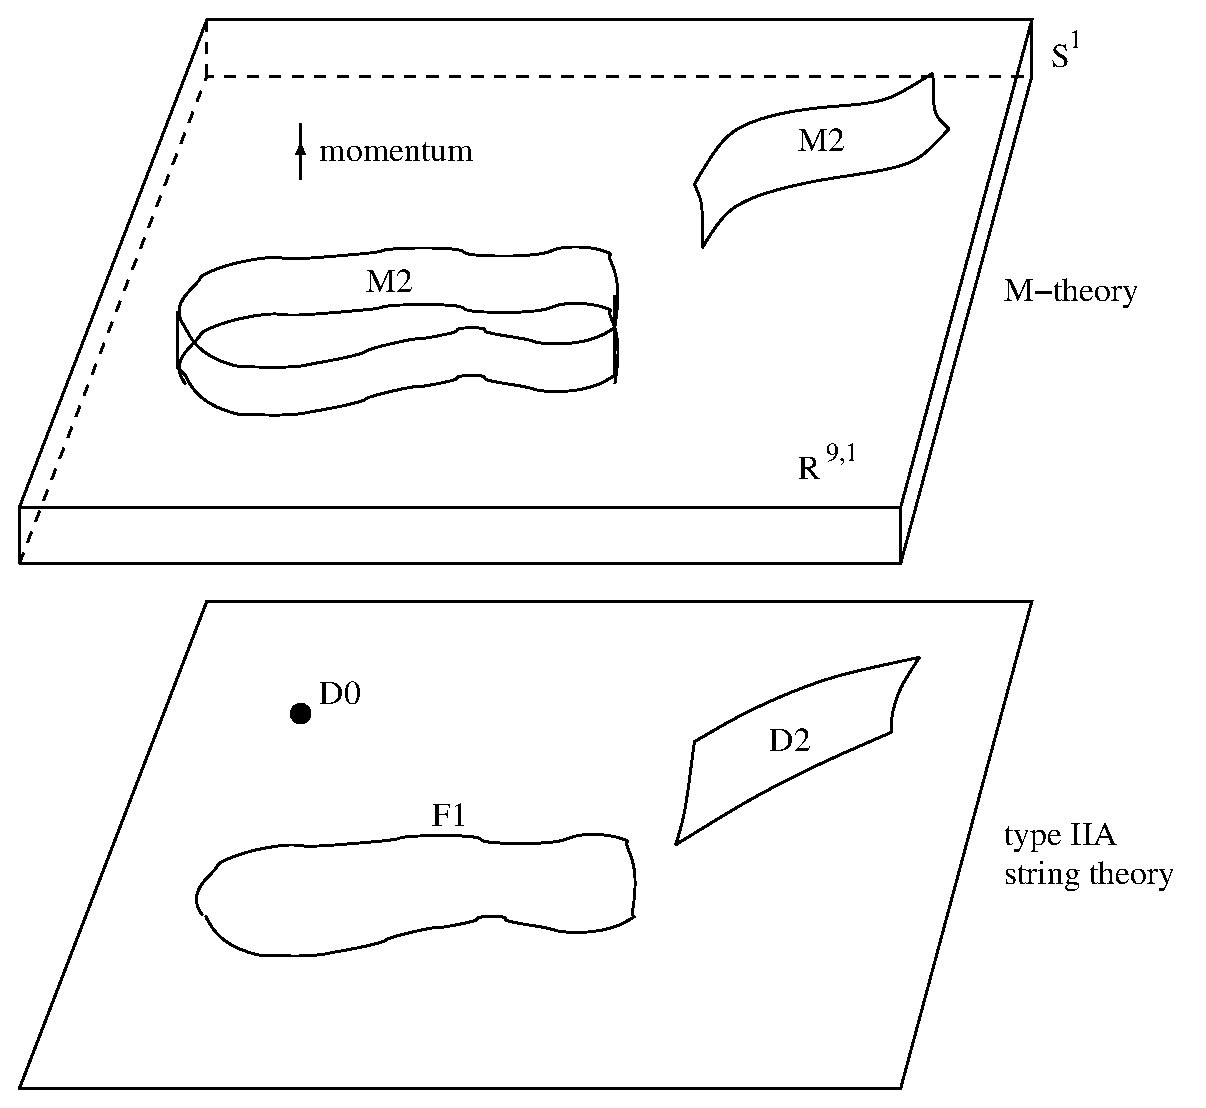
\includegraphics[width=8.0cm]{R91.eps}
\end{center}
\caption{Dimensional reduction of M-theory}
\label{Mreduction}
\end{figure}


The M2 and M5 tensions are proportional to the single energy scale $M_p$, $T_{M2} \propto M_p^3$ and $T_{M5} \propto M_p^6$.  
Originally M-theory has no dimensionless parameter, but from dimensional reduction of IIA one can get a dimensionless parameter $g_s$, the string coupling constant,
\ba
g_s^{2/3} & \propto & M_p R_{10} \\
g_s & \propto & (M_p R_{10})^{3/2}
\ea
where $R_{10}$ is the radius of $S^1$.
The M-theory is obtained as follows. 
In flat spacetime, M2 world volume action is
\be \label{Maction}
S_{M2} ~~=~~ M_p^3 \int d^3 \sigma \sqrt{{\rm det}G_{\mu\nu}}\, (C_{IJK}\epsilon^{\mu\nu\lambda}\partial_\mu X^I \partial_\nu X^J \partial_\lambda X^K).
\ee
One quantizes its Polyakov version, similarly to how it is done in string theory, then it yields a complicated interacting theory. 
A discretization leads to Matrix model and the spectrum becomes discrete. 
Bank, Fisler, Shenker and Susskind did the same thing from relation to IIA theory, where they found a continuous spectrum as the theory was 2nd quantized \cite{BFSS,Tayl}. 
We will consider M-theory on $AdS_4 \times S^7$ which should have non-perturbative description from a decoupled theory on M2-branes.

\section{M-theory on $AdS_4 \times S^7$}

One approach to M-theory is a direct quantization of Polyakov version of action similar to eq. \eqref{Maction} a flat background. 
In this section we will consider an AdS/CFT dual description, which is believed to be successful until now, and will provide understanding of non-perturbative aspects of 
the theory.
Precisely, low-energy physics on coincident M2-branes can give a non-perturbative description of M-theory on $ AdS_4 \times S^7 $.
\begin{center}
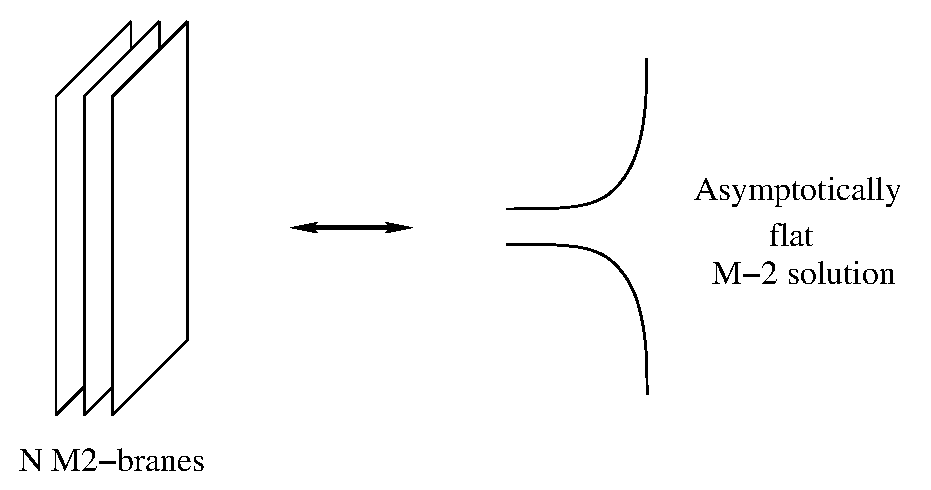
\includegraphics[width=8.0cm]{throat1.eps}
\end{center}
The geometry is described by the metric 
\begin{align*}
	ds^2 & ~~=~~ H^{-2/3}(r)\, dx_\mu dx^\mu ~~+~~ H^{1/3}(r) \left(dr^2 ~+~ r^2 d\Omega_7^2 \right) \\
	H(r) & ~~=~~ 1 ~~+~~ \frac{32\pi^2 N_{M2} l_p^6}{r^6}~.
\end{align*}
One can send supergravity modes and calculate the absorption cross-section given the energy $ \omega $:
\[
	\sigma_{M2} ~~\propto~~ \omega^2 N^{3/2} l_p~, \qquad\qquad l_p ~=~ 1/M_p~.
\]
It can be seen that the cross-section tends to zero as $ \omega \to 0 $, i.e slow particles would not notice the black hole.
Still there is interesting physics in near-horizon region, consider energy
\[
	E ~~=~~ \epsilon M_p~, \qquad  \epsilon ~\to~ 0~.
\]
Focus on the region of $ r $ such that local energies of order $ M_p $ get redshifted to energies of order $ \epsilon M_p $ as viewed
from infinity.
The result is 
\[
	H ~~\to~~ \frac{2^5 \pi^2 N_{M2} l_p^6}{r^6}~.
\]
In $ AdS_4 \times S^7 $ this is a maximally supersymmetric solution of 11-dimensional supergravity.

In the brane picture, in the limit $ E/M_p \to 0 $ one should observe some interesting worldvolume theory which is 
decoupled from the asymptotical physics, and dual to $ AdS_4 \times S^7 $ M-theory, with
\[
	R_{S^7} ~~\sim~~ R_{AdS} ~~\sim~~ N^{1/6} l_p~.
\]
To obtain the supergravity limit, one takes $ N \to \infty $ which yields 11-dimensional supergravity.

The geometry of $ AdS_4 \times S^7 $ has the symmetry group OSp(8$|$4) which breaks up as follows:
\begin{center}
\begin{tabular}{llll}
			     &  \parbox{3.0cm}{\small\centering SO(3,2)\\ {\small symm of $AdS_4$}} & $ \Rightarrow $ & conformal field theory \\[1mm]
bosonic:		     &  \parbox{3.0cm}{\small \centering $ \times $} \\
                             &  \parbox{3.0cm}{\small\centering SO(8)\\ {\small symm of $ S^7 $}} & $ \Rightarrow $ & SO(8) global symmetry \\[5mm]
			     &  \parbox{3.0cm}{\small\centering 16 generators commute with $P_\mu$}  & $ \Rightarrow $ & $ \mc{N}=8 $ supersymmetry \\[1mm]
fermionic:		     &  \parbox{3.0cm}{\small \centering $ \times $} \\
			     &  \parbox{3.0cm}{\small\centering 16 other generators} & & (from superconformal algebra)
\end{tabular}
\end{center}

On the CFT side, the spectrum of these operators must match with the states of M-theory on (global) $ AdS_4 \times S^7 $.
These states are known only for $ N \to \infty $:
\[
	\raisebox{-2.0mm}{\parbox{2.0cm}{\small\centering low dim operators}} ~~\underleftrightarrow{N \to \infty} 
	\raisebox{-1.0mm}{\parbox{3.0cm}{\small\centering spectrum of supergravity modes}}
\]
The question of finding the spectrum reduces to the question of determining which representation of OSp(8$|$4) there is.
One can generate these states starting from a finite number of states of the lowest energy (i.e. lowest dimensional operators)
and acting with symmetry generators
\[
	\text{supergravity modes} ~~\to~~ \parbox{5.0cm}{\centering lowest dim operators, ``chiral primary operators''.}
\]
These operators are in symmetric traceless representation of SO(8):
\[
	\mc{O}^{I_1 \dots I_n} ~, \qquad \delta_{IJ}\mc{O}^{I_1 \dots I \dots J \dots } ~~=~~ 0~,
\]
and their dimension equals $ n / 2 $ where $n$ is the number of indices.
Another piece of information is that 3-point functions of the Chiral Primary Operators are known at large $ N $.

In M2-brane theory, one should be able to bring apart the M2-branes, and then the moduli of the M-theory should correspond to the positions of these
N identical objects in $ \mc{R}^8 $.
Therefore, the moduli space is $\left( \mc{R}^8 \right)^N / S_N $, with $ S_N $ being the permutation group of the positions of M2-branes.

%$AdS_4 \times S^7$ has its symmetry group OSp(8$|$4) $\sim$ SO(2,3) $\times$ SO(8), and which correspond to 3 dim. conformal group and SO(8)$_R$ global symmetry. Supersymmetric point of view, this is Bosonic part. Fermionic part has 16 conventional supersymmetric generator which commute with $P_\mu$ and it gives $\calN$ = 8 susy. The number of non-conventional supercharge is also 16.
%
%Spectrum of CFT operators in $R \times S^2$ must match with states of M-theory on global $AdS_4 \times S^7$. Especially low energy limit of 11d supergravity which is equal to the large N limit, low dimensional operators in CFT, chiral primary operator, matches with spectrum of supergravity modes. There sit in representations of OSp(8$|$4). M2 brane theory should have moduli space correspond to positions of N identical brane in $\mathrm R^8$, its moduli space is $(\mathrm R^8)^N/S_N$. 

One can write down a Lagrangian with the simplest multiplet, 8 scalars + 8 fermions, in an $\calN$=8 theory.
This corresponds to a single M2-brane, i.e. a free theory. 
In $\calN$=1 language, 
\be
\calL=-\frac{1}{2}\partial_\mu X^I \partial^\mu X^I + \frac{i}{2} \ov{\Psi}^a \gamma^\mu \partial_\mu \Psi^a~.
\ee
What would be an interacting theory of an M2-brane? 
By dimensional reduction of $\calN$=4 U(N) supersymmetric Yang-Mills theory, one can obtain a D2-brane theory in 2+1 dimensions with $\calN =8 $ supersymmetry,
\be \label{proto1}
\calL ~~=~~ \frac{1}{g_{YM}^2} \mathrm{Tr}\lgr-\frac{1}{4} F_{\mu\nu} F^{\mu\nu} - \frac{1}{2}D_\mu X^I D^\mu X^I + \frac{1}{4} [X^I, X^J]^2  + {\mathrm{fermions}}\rgr~.
\ee
This is a 2+1-dimensional $\calN=8$ theory which is not conformal since it contains a dimensionful parameter $g_{YM}$!
Indeed, writing the action schematically as,
\be
\int d^3 x \left(\partial A \partial A +\partial A A A + A A A A \right).
\ee
one observes that the gauge field $ A_\mu $ has mass dimension one, and therefore the coupling constant should have mass dimension one as well. 
Such a theory has a non-trivial RG flow.
How does it behave in the infrared?
This theory is \underline{believed} to have a 2+1-dimensional SYM superconformal fixed point (and the latter is the M2-theory).

To determine the moduli space, consider the vacuum configuration of \eqref{proto1}. 
The potential vanishes when all $X^I$'s commute, i.e. they should be diagonal up to a gauge transformation. 
At a generic point the U(N) is broken into diagonal U(1)'s, U(N) $\rightarrow$ U(1)$^N$.
These U(1) gauge fields can be dualized to scalars in 2+1 dimensions, $A_\mu \leftrightarrow \phi$:
\begin{itemize}
\item add Lagrange multiplier $\int d^3x \frac{\sigma_n}{8 \pi} \partial_\mu F_{\nu\lambda}^n \epsilon^{\mu\nu\lambda}$ to impose 
	Bianchi identity and F to be treated as an independent variable.
\item integrate out $F_{\mu\nu}^n$
\item this gives the usual kinetic term, $g^2_{YM} \partial_\mu \sigma_n \partial^\mu \sigma^n$
\end{itemize}
The field $\sigma_n$ has a period of $2\pi$, which is related to monopole configurations. 
For a gauge field with a monopole configuration $\int_{\mathcal M}$dF = $\int_{\partial \mathcal M} F \in 4 \pi Z$. 
A shift by $2\pi$ of $\sigma_n$, shifts the action by 2 $\pi$, but in the path integral exp(i S) is invariant. 
The moduli space of this theory is $(\mc{R}^7 \times S^1)^N/S_N$.  The scalar VEVs are $X^I = diag(a_1^I, a_2^I,\cdots,a_N^I)$.
The radius of $S^1$ is proportional to $g_{YM}$, which can be obtained by canonically normalizing $\sigma_n$. 
This matches the M2-brane theory moduli space when $g_{YM}^2$ goes to infinity or in the IR limit with $g_{YM}^2$ fixed.
Summarizing, M2-theory has following properties.
\begin{center}
\begin{tabular}{|c|c|ccc|}
\hline
Symmetry & OSp(8$|$4)           & SO(2,3) & AdS$_4$   & 2+1 CFT \\
                 & $\calN$=8 susy      & SO(8)    & $S^7$       & SO(8)$_R$ \\
\hline
Moduli space & \multicolumn{4}{c|} {$(R^8)^N/S_N$}\\
\hline
number of d.o.f.     & \multicolumn{4}{c|} {$N^{3/2}$}\\
\hline
\end{tabular}
\end{center}
One conjectures that M2-brane theory could be  some gauge theory where $N$ is associated with the rank of the gauge group. 
From the above example, one may get an explicit description of M2-brane theory. 
The claim is that the type IIA D2-brane theory has an IR fixed point which provides an M-theory description. 
The M2-brane theory should be a 2+1-dimensional SYM with conformal symmetry, but the YM term is not scale invariant in 2+1 dimensions. 
A possible candidate of such a theory is the Chern-Simon theory \cite{Dunne}. 

\section{Chern-Simons theory}

An example of 2+1-dimensional CS theory with the gauge group U(N) is 
\be
S ~~=~~ \frac{k}{4 \pi} \int d^3 x \epsilon^{\mu\nu\lambda} {\rm tr}\left(A_\mu \partial_\nu A_\lambda + \frac{2i}{3} A_\mu A_\nu A_\lambda \right).
\ee
Under an infinitesimal variation of $A_\mu$,
\be
\delta S ~~=~~ \frac{k}{4 \pi} \int d^3 x \epsilon^{\mu\nu\lambda} {\rm tr}\left(\delta A_\mu F_{\nu\lambda} \right).
\ee
where $F_{\mu\nu}=\partial_\mu A_\nu - \partial_\nu A_\mu +i [A_\mu,A_\nu]$.
If one takes an infinitesimal gauge transformation $\delta A_\mu = D_\mu \Lambda = \partial_\mu \Lambda + i [A_\mu, \Lambda]$,
the action variation vanishes by Bianchi identity, $\epsilon^{\mu\nu\lambda}D_\mu F_{\nu \lambda} =0 $.

To consider large gauge transformations, we define the transformation matrix $U(x)$ which acts on gauge field, 
$A_\mu \rightarrow U(x) A_\mu U(x)^{-1}+ i \partial_\mu U(x) U(x)^{-1}$. 
The change of action due to this transformation is $ S \rightarrow S - 2 \pi  w(U) $, where 
\[ 
w(U)~~=~~ \int d^3 x \frac{1}{24 \pi^2} \epsilon^{\mu\nu\lambda} tr (U^{-1}\partial_\mu U U ~ U^{-1}\partial_\nu U U ~U^{-1}\partial_\lambda U U)~.
\] 
The $ w(U) $ is a topological invariant similarly to the instanton number $\int tr(F\wedge F)$, and both of them are integers. 
Let $w(U)$ be $n$, $n \in Z$, then the action variation is $2 \pi k n$. 
For integer $k$, $e^{i S}$ is invariant under all gauge transformations. 
In 2+1 dimensions the CS theory has no dimensionful parameters, so it can potentially be part of a CFT.
But CS action does not involve the metric, and therefore it is a topological field theory with no propagating degrees of freedom. 
However, it can still couple to matter.\\

\noindent\underline{\large \it Parity}\\
Under the parity transformation, $S^k_{CS}(A) \rightarrow -S^k_{CS}(A)$ \footnote{hereafter, let $k$ be the level of the CS theory.}, and so CS is not parity invariant. 
However, the difference  $S^k_{CS}(A) -S^k_{CS}(\tilde{A})$ is parity invariant, if one introduces new parity operation  $x \rightarrow -x $ accompanied by $A \rightarrow \tilde{A}$.\\

\noindent\underline{\large \it Supersymmetric CS theory}\\
Does Chern-Simons theory have a supersymmetric extension? 
As a theory of M2-brane, it should. 
Many authors address this question, and find interesting results. 
For $ \mc{N}=1,2,3 $ the superfield method is available to build Lagrangians for any gauge group and matter representations.
An $ \mc{N}=3 $ theory in 2+1 dimensions is conformal.
For the $\calN =4 $ case, only specific gauge groups U(N) $\times$ U(M) or O(N) $\times$ SP(M) with bifundamental matter were found \cite{GW}
\begin{center}
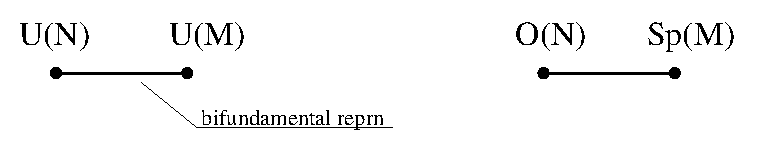
\includegraphics[width=9.0cm]{bifund.eps}
\end{center}
There is more progress in quiver gauge theory by Hosomichi, Lee, Lee, Lee, Park \cite{HL3P}, where they were able to generalize to
\begin{center}
\includegraphics[width=9.0cm]{hosomichi.eps}
\end{center}
or a cyclic version.
The fact the latter one has $ \mc{N}=4 $ is manifest in $ Q_\alpha^i $, which are rotated by the SO(4) subgroup of the R-symmetry group:
\begin{center}
\begin{tabular}{lcc}
	$SO(4)$ & ~~$\sim$~~ & $SU(2) \times SU(2)$ \\
        hypermt & & $ q_\alpha \qquad \psi_{\dot{\alpha}}$ \\
	twisted hypermt && $ \wt{q}_{\dot{\alpha}} \qquad \wt{\psi}_\alpha  $ ~,
\end{tabular}
\end{center}
Here the first SU(2) rotates $ q_\alpha $ and $ \wt{\psi}_\alpha $, while the other one rotates
$ \wt{q}_{\dot{\alpha}} $ and $ \psi_{\dot{\alpha}} $.

The ABJM U(N)$\times$ U(M) theory 
\begin{center}
\includegraphics[width=4.0cm]{abjm_u.eps}
\end{center}
has $\calN =6 $ supersymmetry, and in the $N=M=2$ case 
\begin{center}
\includegraphics[width=4.0cm]{abjm_su.eps}
\end{center}
supersymmetry is enhanced to $\calN=8 $ with a three-algebra structure. 
Bergman-Lambert theory \cite{BL} fits into this, as shown in \cite{HL3P}.
But the SU(2)$\times$SU(2) theory is not matched to M2 theory, because the moduli space is different. 
Its moduli space is $R^8 \times R^8 /D_{2k}$, $D_{2k} \sim Z_2 \ltimes Z_k$. 
However, in the case of $ k = 1,2 $ and $3 $, it coincides with the moduli space of SO(4), SO(5) and $ G_2 $ 2+1-dimensional SYM.
Therefore $ k $ has to do with orbifolding in ABJM.
They proposed that $ \mc{N}= 6 $ supersymmetry is enough:
{\it $\calN$=6  U(N)$\times$ U(N) theory at level k is equivalent to the low energy dynamics of coincident N M2-branes theory on $\mc{R}^8/Z_k$} \cite{ABJM}. 
And it is dual to the M-theory on $AdS_4 \times S^7 /Z_k$.
The case of $k=1 $ is special in that M-2 theory on $ \mc{R}^8 $ predicts $ \mc{N}=8 $ supersymmetry since there is no orbifolding.
The same is true for $ k = 2 $.\\
%When the level k is 1, this is special case. There is no orbifolding, M2 on $R^8$, it predicts that secret $\calN$=8 symmetry. This is true for k=2, even though $\calN$ = 6 susy is manifest in Lagrangian but 8 is not.\\

\noindent\underline{\large \it ABJM model}\\
This theory has $A_\mu, \tilde{A}_\mu$ U(N) gauge fields and scalars $C^I$  and fermions $\psi^I$.  
$C^I, \psi^I$ are bifundamental matter in fundamental representation of R-symmetry SU(4) $\sim$ SO(6)$_R$. 
The action is
\be
\calL ~~=~~ \calL_{CS}^k(A)- \calL_{CS}^k(\tilde{A}) -V(C, \psi) + {\mathrm Tr}\left(-D_\mu C_I^\dagger D^\mu C^I - i \psi^{I \dagger}\gamma^\mu D_\mu \psi_I \right)
\ee
where $D_\mu C^I = \partial_\mu C^I + i A_\mu C^I - i C^I \tilde{A}_\mu$.  
The potential is
\be \label{ABJMpot}
V ~~=~~ \frac{8 \pi^2}{k^2}\Tr \left(C_I C^{\dagger[I}C_JC^{\dagger J}C_KC^{\dagger K]} - C_I C^{\dagger [I}C_J C^{\dagger K]}C_K C^{\dagger J} \right) + CC\psi^\dagger\psi {\rm terms}~.
\ee
One can explicitly write down  $\calN$=6 supersymmetry transformation for any $k$. 
All terms are dimension 3 so this theory is conformal at least at the classical level.
Since $k$ is discrete there is no continuous renormalization. 
This means that for large $k$ the theory is weakly coupled.

This is confirmed by the moduli space. 
The potential \eqref{ABJMpot} vanishes when $C^I$ are diagonal, while at a generic point U(N)$\times$U(N) is broken to U(1)$^N$: 
\be
C^I ~~=~~ \left(\begin{array}{ccc}
z_1^I&&\\
&\vdots&\\
&&z_N^I 
\end{array}
\right)
, ~~ 
A_\mu = \left(\begin{array}{ccc}
a^1_\mu&&\\
&\vdots&\\
&&a^N_\mu
\end{array}
\right)
,~~
\tilde{A}_\mu= \left(\begin{array}{ccc}
\tilde{a}^1_\mu&&\\
&\vdots&\\
&&\tilde{a}^N_\mu 
\end{array}
\right)
\ee
Then the light degrees of freedom are described by
\be
\calL~~=~~\frac{k}{4\pi}\epsilon^{\mu\nu\lambda}(a^n_\mu \partial_\nu a^n_\lambda- \tilde{a}^n_\mu \partial_\nu \tilde{a}^n_\lambda)-
			|\partial_\mu z_n^I + i(a^n_\mu-\tilde{a}^n_\mu)z^I_n|^2 + ~{\mathrm{fermion}}+~{\mathrm{massive}}~.
\ee
Let  $b_\mu^n=a^n_\mu-\tilde{a}^n_\mu$ and $c_\mu^n=a^n_\mu+\tilde{a}^n_\mu$, in terms of which the Lagrangian is
\be
\calL~~=~~\frac{k}{8\pi}\epsilon^{\mu\nu\lambda}b_\mu^n F_{\nu\lambda}^n -|\partial_\mu z_n^I + i b^n_\mu z^I_n|^2 
\ee
One again introduces the Lagrange multiplier via $\frac{1}{8\pi}\sigma_n\epsilon^{\mu\nu\lambda} \partial_\mu F_{\nu\lambda}^n$ and treats $F$ as an independent variable. 
The field strength $F$ can be integrated out. It follows that $b_\mu = \frac{1}{k}\partial_\mu \sigma$. 
The Lagrangian now reduces to
\be
\calL~~=~~-|\partial_\mu z_n^I + \frac{i}{k} z^I_n \partial_\mu \sigma|^2 
\ee
Under the gauge transformations $b_\mu^n \rightarrow b_\mu^n -\partial_\mu \alpha_n(x) $, $z_n^I \rightarrow e^{i \alpha(x)} z_n^I$ and $\sigma_n \rightarrow \sigma_n - k \alpha_n(x)$. 
Choosing proper $\alpha$, one can always set $\sigma$ = 0 and the residual gauge transformation will be $\alpha = 2\pi n /k$. 

The dynamics of moduli fields is given by $-|\partial_\mu z_n^I |^2$ with the residual gauge transformation $z_n^I \rightarrow e^{i 2\pi n /k} z_n^I$. 
Each diagonal element contributes $R^8/Z_k$. Still there is symmetry permuting $ z_n $, so the moduli space is $(R^8/Z_k)^N/S_N$, where $S_N$ is symmetrization.
Thus, ABJM passes the moduli space test.

What happens at large $ k $?
$ S^7 $ can be considered a $ S^1 $ fibration over $ CP^3 $. 
$ Z_k $ acts on this circle $ S^1 $.
For large $ k $ one needs a circle with a small radius, and therefore one effectively has a dual to a type IIA string on
$ AdS^4 \times CP^3 $.
In the type IIA picture,
\[
	\frac{R^4}{(\alpha')^2} ~~=~~ \frac{N}{k} ~~\sim~~ \lambda~.
\]
The other parameter is the string coupling
\[
	g_s ~~\sim~~ \lambda^{5/4} \frac{1}{N} ~~=~~ \left( \frac{N}{k^5} \right)^{1/4}~.
\]
If $ k $ is too large, then $ R $ is too large(?)
\begin{center}
\includegraphics[width=10.0cm]{lambda.eps}
\end{center}


\underline{Now we resort back to $ k = 1 $} and check that this theory has the right spectrum of chiral primary operators
\begin{center}
\begin{tabular}{cccc}
%
	$ \mc{O}^{i} $   & $ \mc{O}^{ij} $  &  $ \mc{O}^{ijk} $  & $ \dots $ \\
%
	{\small dim $\frac{1}{2} $}    &  {\small dim $ 1 $}     &  {\small dim $ \frac{3}{2} $} & \dots
\end{tabular}
\end{center}
with SO(8) acting upon them.
In ABJM theory, only the SU(4) symmetry is manifest. 
Actually, it is the $ SU(4) \times U(1) \subset SO(8) $ which is explicit: SU(4) rotates the $ C^I $, while the U(1) does a phase
rotation $ C^I \to e^{i\theta} C^I $.
Naively, the latter is the gauge symmetry associated with the abelian field
\[
	b_\mu ~~=~~ a_\mu^{U(1)} ~-~ \wt{a}_\mu^{U(1)}~.
\]
However, there is a Chern-Simons term in the Lagrangian
\[
	\frac{k}{4\pi} \epsilon^{\mu\nu\lambda} b_\mu f^{(c)}_{\nu\lambda} ~, 
\]
where $ f^{(c)}_{\mu\nu} $ is a fieldstrength associated with $ c_\mu = a_\mu + \wt{a}_\mu $.
That means that the charge operator of $ b^\mu $ is not only built of matter, but also of $ c^\mu $:
\be
\label{Qsum}
	Q_{\rm matter}^{U(1)} ~+~ k \int \frac{1}{4\pi} \epsilon^{0\mu\nu} f_{\mu\nu}^{(c)}~.
\ee
This brings a modification into the Gauss theorem.
For example, what are the allowed states of the theory on a sphere? 
Net charge is not allowed on a compact space. 
$ C^I $ and $ C_I^\dag $ create positive and negative charge particles, and
therefore the sum of the charge must vanish.
In our case, the sum \eqref{Qsum} must vanish, i.e.
\[
	Q ~~=~ k\, \int_{S^2} \frac{1}{4\pi} \wt{f}{}^{(c)} ~~\Leftarrow~~ \text{units of magnetic flux on the sphere}~,
\]
\begin{center}
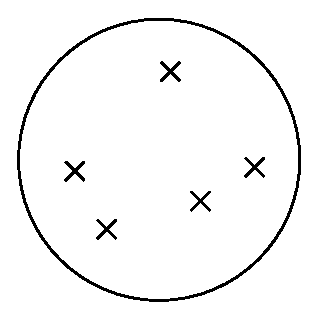
\includegraphics[width=2.5cm]{sphere.eps}
\end{center}
With $ n $ units of magnetic flux, we can have $ k \cdot n $ units of U(1) charge.
In a sense this $ U(1) $ is then ``global''.
Let us try to write down chiral primary operators.
For example, the dimension one operator
\[
	\mc{O}^{ij} ~~\to~~ \text{splits into representations}~ \left(\mc{O}^I_J\right)_0 ~, \left(\mc{O}^{IJ}\right)_2 ~,  \left(\mc{O}_{IJ}\right)_{-2}
\]
under $ SO(8) \to SU(4) \times U(1) $, with 0, 2 and -2 indicating the U(1) charges.

Start with $ \left(\mc{O}^I_J\right)_0 $, adjoint of SU(4). 
This one has charge 0, and therefore should be composed of an equal number of $ C^I $ and $ C_I^\dag $. 
One only can use one $ C^I $ and one $ C_I^\dag $:
\[
	\mc{O}^I_J ~=~ tr \lgr C^I C_J^\dag ~-~ \frac{1}{4} \delta^I_J C^K C_K^\dag \rgr~.
\]
Now consider $ \left(\mc{O}^{IJ}\right)_2 $: one needs two $ C^I $ and no $ C_I^\dag $'s:
\[
	tr \left( C^I C^J \right )  \text{ is not gauge invariant, as} \quad C ~~\to~~ U\, C\, V^\dag~.
\]
Recall the connection between the operators and the states of gravity:
\[
	\parbox{4.0cm}{\centering local operators\\ on $ R^3 $} ~~\leftrightarrow~~
	\parbox{3.0cm}{\centering states on\\ $ S^2\times \mc{R} $} 
\]
For $ k = 1 $ one can have a state with two $ C^I $'s as long as there are two units of flux, and hence
there is a corresponding local gauge-invariant operator.
It should be analogous to magnetic flux.
There is such an operator which is called the {\it 't Hooft disorder operator} \cite{'tHooft:1977hy},
and associated with creation of flux.
For $ k = 2 $ one needs two $ C^I $'s and hence one unit of magnetic flux.  
For $ k > 2 $ one cannot have a charge 2 state.

Summarizing, for $ k=1 $ and $ k=2 $ one is able to write the corresponding operators, and therefore
the realization of SO(8) is only possible for these values of $ k $.

As a general approach, one can think of an operator $ T_{\dot{b}_1\dots\dot{b}_k}^{a_1\dots a_k} $ in
$ \left( Sym(N^k), Sym(\ov{N}^k) \right) $ representation of U(N)$\times$U(N):
\begin{center}
\begin{tabular}{lll}
  $ k = 1 $:\qquad   & one can choose $ T^a_{\ \dot{b}} $,  & and write down $ tr \left(C^I T C^J T \right) $ \\
  $ k = 2 $:\qquad   & four-index $ T^{ab}_{\dot{a}\dot{b}} $, & and the operator $ C^{I\;\dot{a}}_a C^{J\;\dot{b}}_b T^{ab}_{\dot{a}\dot{b}} $
\end{tabular}
\end{center}

\section{Relation to 3-Algebras}

There is a supersymmetric configuration in string theory
\begin{center}
\includegraphics[width=5.0cm]{D1D3.eps}
\end{center}
which looks as a magnetic monopole on D3 branes.
Associated, there is a solution where D1's expand
\begin{center}
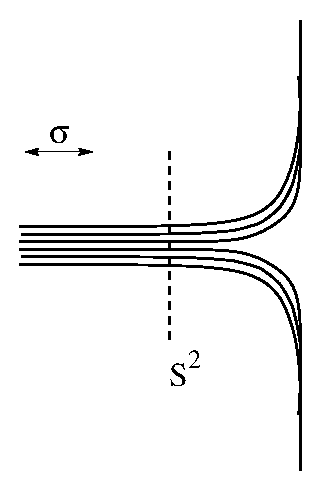
\includegraphics[width=3.0cm]{fuzzy.eps}
\end{center}
known as ``fuzzy funnels''.
In terms of fields, this cross-section should be a sphere, by symmetry
\begin{align*}
	X^i(\sigma) & ~~=~~ R(\sigma) X_0^{\ i}  \\
	[ X_0^{\ i} \, X_0^{\ j} ] & ~~=~~ i \epsilon^{ijk} X_0^{\ k}~,
\end{align*}
with $ X_0^{\ i} $ being $ N\times N $ matrices.
This is a non-commutative algebra representing a fuzzy 2-sphere.

There is another example due to Basu and Harvey \cite{Basu:2004ed} 
\begin{center}
\includegraphics[width=4.5cm]{M2M5.eps}
\end{center}
who suggested that such a field theory should have similar funnel configurations.
By symmetry, the cross-section of such a configuration should be a $ S^3 $: four directions
on M5 which are orthogonal to the M2-brane.
For a fuzzy 3-sphere one needs an equation similar to
\[
	\left[ X_0^{\ i} \, X_0^{\ j} \, X_0^{\ k} \right] ~~=~~ f^{ijkl} X_0^{\ l}~.
\]

\subsection{3-Algebras}

Bagger, Lambert \cite{BL} and Gustavsson \cite{Gus} suggested to try to build a theory based
on 3-algebras:
\begin{itemize}
\item
	start with some vector space, endowed with a basis $ T^a $
\item
	introduce the triple product for the generators:
\[
	[ T^a\, T^b\, T^c ] ~~=~~ f^{abc}_{\ \ \ d} T^d
\]
	and a norm $ \left\langle T^a \, T^b \right\rangle ~=~ h^{ab} $.
\item
	they constructed an $ \mc{N}=8 $ supersymmetric Lagrangian for any structure $ f^{abc}_{\ \ \ d} $ such that
\begin{itemize}
	\item
	$ f^{abcd} ~=~ h^{de} f^{abc}_{\ \ \ e} $ should be totally antisymmetric
	\item
	generalization of Jacobi identity: the bracket should act like a derivative
\[
	\left[ A\, B \, \left[ C\, D \, E \right]\right] ~~=~~
	\left[ \left[ A\, B \, C \right] D\, E \right] ~~+~~ \left[ C\, \left[ A\, B\, D \right] \, E \right] 
	~~+~~
	\left[ C\, D\, \left[ A\, B\, E \right] \right] 
\]
\end{itemize}
\end{itemize}
Take fields valued in this algebra
\begin{center}
\begin{tabular}{llll}
   $ X_a^I T^a $  & --- 8 scalars &  \qquad\qquad $ A^\mu_{ab} $ & --- gauge field, antisymm in $(ab)$ \\
   $ \psi_{\alpha\, a} $  & --- 8 fermions.
\end{tabular}
\end{center}
The Lagrangian contains the CS term
\[
	\frac{1}{2} \epsilon^{\mu\nu\lambda} 
		\lgr f^{abcd} A_{\mu\,ab} \p_\nu A_{\lambda\, cd} ~+~
			\frac{2}{3} f^{cda}_{\ \ \ g} f^{efgb} A_{\mu\, ab} A_{\nu cd} A_{\lambda ef} \rgr
\]
The matter fields couple to the ``dual'' potential
\[
	\wt{A}{}_{\mu\ d}^{\ c} ~~=~~ f^{abc}_{\ \ \ d} A_{\mu\, ab}
\]
via the covariant derivative
\[
	\md_\mu X_a^I ~~=~~ \p_\mu X_a^I ~+~  i\, (\wt{A}{}^{I} X)_a~.
\]
One introduces the kinetic terms 
\[
	h^{ab}\, \md_\mu X_a^I \md^\mu X^I_b  ~~+~~ h^{ab}\, \ov{\Psi}{}_a \Gamma^\mu \md_\mu \Psi_b
\]
and the potential 
\[
	\left\langle [X^I\, X^J\, X^K ] , [X^I\, X^J\, X^K ] \right\rangle ~~+~~
	\left\langle \ov{\Psi}, \Gamma^{IJ} [ X^I\, X^J \, \Psi ] \right \rangle~.
\]
Unfortunately, there is only one example of a 3-algebra with positive-definite $ h^{ab} $:
%\begin{center}
\[
\parbox{3.0cm}{\centering\small 4-dimensional space}
\qquad
\left\{~~
\parbox{2.5cm}{$ h^{ab} ~~=~~ \delta^{ab} $ \\$ f^{abcd} ~~=~~ \epsilon^{abcd} $ }
\qquad
\parbox{1.0cm}{$ \Rightarrow$}
\qquad
\parbox{6.0cm}{\small ordinary gauge theory, SU(2)$\times$SU(2) $ \mc{N}=8 $ CS theory,
				which does not suit the purpose due to its complicated moduli space.}
\right.
\]
Another example exists with Lorentzian metric: 
\[
\left\{~~
\parbox{5.0cm}{
$ h^{+-} ~=~ 2 \qquad h^{ab} ~=~ \delta^{ab} $  \\
{\small (in light-cone variables)} \\
$ f^{abc+} ~=~ f^{abc} $
}
\right.
  \qquad\text{with $ f^{abc} $ structure constants for any Lie algebra}
\]
With such a metric one inevitably has negative norm states.
The usual method of adding Faddeev-Popov ghosts can be applied.
However, in the trivial vacuum $ \langle X^I \rangle = 0 $ the resulting BRST theory is equivalent to a
free theory.
If one gives $ X^I $ a VEV, the theory becomes equivalent to $ \mc{N}=8 $ 2+1-dimensional SYM 
with $ g_{YM}^2 = v^2 $.

Bagger and Lambert \cite{BL} suggest that they can reproduce $ \mc{N}=6 $ theories, including ABJM,
by allowing the structure constants $ f^{abcd} $ to be complex and relaxing the constraints
\begin{align*}
&	f^{ab;cd} ~~=~~ -\, f^{ba;cd} ~~=~~ (f^{cd;ab})^* ~~=~~ -\,f^{ab;dc} \\
&	\left[ C \left [ E \, F \, G \right] A \right] ~~-~~
	\left[ C \left[ E \, F \, A \right] G \right] ~~=~~
	\left[ C \, E \left[ A\,G\,F \right]\right] ~~-~~ \left[ C\,F \left[ A\, G \, E \right] \right]~.
\end{align*}

\subsection{Interesting generalizations}
\begin{itemize}
\item U(N)$\times$U(M) theory \cite{Aharony:2008gk}: M2 branes on $ \mc{R}^8/Z_k $ and fractional M2 branes
\item
	M-2 theory on $ T^2 $: DLCQ description of type IIB strings on flat space
\item
	``BMN'' sector should give M-theory on 11-dimensional plane wave, i.e. a large $N$ plane wave Matrix Model
\item
	there exists maximally supersymmetric mass deformations of the theory which preserve SO(4)$\times$SO(4),
	and has discrete vacual dual do bubbling geometries
\item
	there is a mass-deformed theory on $ T^2 $: DLCQ of IIB string theory on plane wave, or orbifolded plane
	wave for $ k> 1$, i.e. a large $ N $ quiver theory
\item
	dimensional reductions?
\end{itemize}


\newpage

\begin{thebibliography}{99}

\bibitem{BL}
{\it Modeling multiple M2's } (th/0611108v3) \\
{\it Gauge Symmetry and Supersymmetry of multiple M2-branes} (arXiv:0711.0955) \\
{\it Comments on Multiple M2-Branes} (arXiv:0712.3738) \\
{\it Three-Algebras and $\calN$ =6 Chern-Simons Gauge Theories} (arXiv:0807.0163) \\
Jonathan Bagger and Neil Lambert
\bibitem{Gus}
{\it Algebraic structures on parallel M2-branes} Andreas Gustavsson  (arXiv:0709.1260)
\bibitem{ABJM}
{\it $\calN$ = 6 superconformal Chern-Simons-matter theories, M2-branes and their gravity duals 
}  Ofer Aharony, Oren Bergman, Daniel Louis Jafferis, Juan Maldacena (arXiv:0806.1218)
\bibitem{Pol}
{\it String theory 1, 2} Polchinski, Cambridge press
\bibitem{WB}
{\it Supersymmetry},  Wess , Bagger
\bibitem{Lyk}
{\it Introduction to Supersymmetry} Joseph D. Lykken (arXiv:hep-th/9612114)
\bibitem{Sohn}
{\it Introducing Supersymmetry} M.F. Sohnius (Phys.Rept.128:39-204,1985)
\bibitem{CJS}
{\it Supergravity Theory in Eleven-Dimensions} E. Cremmer, B. Julia, Joel Scherk (Phys.Lett.B76:409-412,1978)
%\cite{Townsend:1996xj}
\bibitem{Townsend:1996xj}
  P.~K.~Townsend,
  {\it Four lectures on M-theory},
  arXiv:hep-th/9612121.
  %%CITATION = HEP-TH/9612121;%%
\bibitem{BFSS} 
{\it M Theory As A Matrix Model: A Conjecture} T. Banks, W. Fischler, S.H. Shenker, L. Susskind (arXiv:hep-th/9610043)
\bibitem{Tayl}
{\it  M(atrix)Theory: Matrix Quantum Mechanics as a Fundamental Theory} W. Taylor (arXiv:hep-th/0101126)
\bibitem{GW}
{\it Supersymmetric Boundary Conditions in N=4 Super Yang-Mills Theory} (arXiv:0804.2902), 
{\it Janus Configurations, Chern-Simons Couplings, And The theta-Angle in N=4 Super Yang-Mills Theory} (arXiv:0804.2907), 
{\it S-Duality of Boundary Conditions In N=4 Super Yang-Mills Theory}(arXiv:0807.3720) \\
Davide Gaiotto, Edward Witten
\bibitem{HL3P}
{\it N=4 Superconformal Chern-Simons Theories with Hyper and Twisted Hyper Multiplets}
(arXiv:0805.3662), 
{\it N=5,6 Superconformal Chern-Simons Theories and M2-branes on Orbifolds}
(arXiv:0806.4977)\\
Kazuo Hosomichi, Ki-Myeong Lee, Sangmin Lee, Sungjay Lee, Jaemo Park 
\bibitem{Dunne}
{\it Aspects of Chern-Simons theory} Gerald V. Dunne (arXiv:hep-th/9902115)
%\cite{'tHooft:1977hy}
\bibitem{'tHooft:1977hy}
  G.~'t Hooft,
{\it On The Phase Transition Towards Permanent Quark Confinement},
  Nucl.\ Phys.\  B {\bf 138}, 1 (1978).
  %%CITATION = NUPHA,B138,1;%%
%\cite{Basu:2004ed}
\bibitem{Basu:2004ed}
  A.~Basu and J.~A.~Harvey,
  {\it The M2-M5 brane system and a generalized Nahm's equation},
  Nucl.\ Phys.\  B {\bf 713}, 136 (2005)
  [arXiv:hep-th/0412310].
  %%CITATION = NUPHA,B713,136;%%
%\cite{Aharony:2008gk}
\bibitem{Aharony:2008gk}
  O.~Aharony, O.~Bergman and D.~L.~Jafferis,
  %``Fractional M2-branes,''
  arXiv:0807.4924 [hep-th].
  %%CITATION = ARXIV:0807.4924;%%


\end{thebibliography}

\end{document} 